\documentclass[letterpaper,12pt,hidelinks]{article}
\usepackage[authoryear]{natbib}


\usepackage{mathtools, graphicx, authblk, setspace, algorithm, enumerate, listings, url, bm}
\usepackage{subcaption}
\usepackage[english]{babel}
\usepackage[left=1in, right=1in, top=1in, bottom=1in]{geometry}
\setcitestyle{authoryear}
\providecommand{\keywords}[1]{\textbf{{Key Words : }} #1}
\newcommand\numberthis{\addtocounter{equation}{1}\tag{\theequation}}

% \lstset{language=R, % set listings
%     basicstyle=\small\ttfamily,
%     stringstyle=\color{DarkGreen},
%     otherkeywords={0,1,2,3,4,5,6,7,8,9},
%     morekeywords={TRUE,FALSE},
%     deletekeywords={data,frame,length,as,character},
%     keywordstyle=\color{blue},
%     commentstyle=\color{DarkGreen},
% }
\graphicspath{{folder/}{/Users/YaqiongYao/Dropbox/5361proj/Figure/}}
\begin{document}



\title{Random Number Generating using Kernel Density Estimator}
\author{Yaqiong Yao, Cheng Huang}
\maketitle



\begin{abstract}
The purpose of this project is to improve the method of drawing samples from an unknown distribution if we have a sample dataset. We are going to introduce kernel density estimate to estimate the cumulative density function of the given dataset. Then sample data from the estimated pdf. This method can be applied to both univariate samples and multivariate samples which are constraint by copulas. 
\end{abstract}

\section{Introduction}

Draw samples from a set of given observed data $\{x_i\}_{i=1}^n$ with unspecified distribution is widely used especially in bootstrap and is still a topic needing pay attention to. \cite{efron1979} came up with the idea of bootstrap and they proposed to use observations randomly selected from $\{x_i\}_{i=1}^n$ with replacement as a sample to inspect the features of the unknown distribution. \cite{kde} introduced the idea of using kernel density estimate (KDE) to draw samples from. In this project, our method is based on the idea of implementing KDE, estimating the cumulative density function of the unknown distribution to take samples and we are going to extend the idea to multivariate samples linked by copulas.

The structure of this project is presented as following. In section 2, we introduce our methodology of taking samples and present the numerical simulations in Section 3.

\section{Methodology}\label{sec:meth}

\subsection{Univariate Case}

Given samples $\{x_i\}_{i=1}^n$ from an unknown distribution, the method proposed by \cite{kde} is first to randomly select values from a pre-specified kernel density and then draw samples from data we have. Adding these two parts together forms the sample we want. They also provided a proof showing that the samples they obtained follow its kernel density estimator (KDE)
\begin{align}\label{eq:kde}
\hat{F}_b(x|\mathcal{D}) = \sum_{i=1}^n \frac{1}{n} K\left(\frac{x-x_i}{b}\right)
\end{align}
where $K(\cdot)$ is the cumulative density function of the selected kernel and $b$ is the bandwidth.

Our method is to obtain the cdf of the KDE explicitly and then randomly sample $u_l \sim \text{Unif}(0,1), l = 1, 2, ... ,N$. Map each $u_i$ to the cdf of KDE and the random samples can be acquired. If we select the uniform kernel, the equation \ref{eq:kde} becomes
\begin{align}\label{eq:kde_uni}
\hat{F}_b(x|\mathcal{D}) = \frac{1}{n}\left\{\sum_{i=1}^n\frac{2x-2x_i+b}{2b} I\left(x_i-\frac{b}{2} < x< x_i + \frac{b}{2}\right) + \sum_{i=1}^n I\left(x \ge x_i + \frac{b}{2}\right) \right\}.
\end{align}
Obviously, this is the a piecewise function with $2n + 1$ intervals and in all intervals, it is a linear function with slop $\frac{n_t}{b}, t = 1,2,...,2n+1$ where $n_t$ is the number of points affecting $t$th interval. Denote $x_t^0$ and $x_t^1$ as the starting point and ending point of $t$th interval. Thus $n_t = \sum_{i=1}^n I(x_i - \frac{b}{2} \le x_t^0 < x_t^1 < x_i + \frac{b}{2})$. Then we can easily draw random samples once all intervals can be obtained. 

We also use the triangular kernel to obtain the kernel density estimate. In this scenario, the equation \ref{eq:kde} is
\begin{align*}
\hat{F}_b(x|\mathcal{D}) = \frac{1}{n} \left\{ \sum_{i=1}^n \int_{x_i - \frac{b}{2}}^x \frac{2b - 4|x-x_i|}{b^2} I\left(x_i-\frac{b}{2} < x< x_i + \frac{b}{2}\right) dx + \sum_{i=1}^n I\left(x \ge x_i + \frac{b}{2}\right) \right\}.
\end{align*}
This is a piecewise function with $3n + 1$ intervals. In each interval, the KDE is in either quadratic form or linear form. The expression for $t$th interval, $t = 1,2, ..., 3n+1$ is $\lambda(x - x_t^0) + \frac{2n_t^*(x^2 - (x_t^0)^2)}{b^2}$, where $\lambda = \sum_{i=1}^n \int_{x_i - \frac{b}{2}}^{x_t^0} \frac{2b - 4|x-x_i|}{b^2} I\left(x_i-\frac{b}{2} < x< x_i + \frac{b}{2}\right) dx$ and $n_t^* = \sum_{i=1}^n I\left(x_i-\frac{b}{2} \le x_t^0 < x_t^1\le x_i \right) - \sum_{i=1}^n I\left(x_i \le x_t^0 < x_t^1 \le x_i + \frac{b}{2} \right)$.



\subsection{Multivariate Case}

In multivariate case, the dependence of random variables are defined by a known copula. Given the observation $\{\bm{\mathrm{x}}_i\}_{i=1}^n$, where $\bm{\mathrm{x}}_i = (x_{1i}, x_{2i}, ..., x_{mi})$ is the value of random variables $x_1, x_2,...,x_m$. With the known copula $C$, the joint probability function is
\begin{align*}
C(u_{1}, u_{2}, ..., u_{m}) = \mathrm{P}(x_{1} \le F_1^{-1}(u_{1}), x_{2} \le F_2^{-1}(u_{2}), ..., x_{m} \le F_m^{-1}(u_{m}))
\end{align*}
where $F_1^{-1},  F_2^{-1}, ..., F_m^{-1}$ are the cdf of every random variable and $u_{1}, u_{2}, ..., u_{m}$ are the marginal probability of each random variable. 

The method of \cite{kde} can be extended to the multivariate case based on a selected kernel density $k(\cdot)$. The procedure is first generate $\bm{\mathrm{e}}_l = (e_{1l}, e_{2l}, ..., e_{ml}), l = 1,2, ..., N$ with each element independently selected from density $k(\cdot)$ and draw observations $\bm{\mathrm{x}}_l^* = (x_{1l}^*, x_{2l}^*, ..., x_{ml}^*)$ from $\{\bm{\mathrm{x}}_i\}_{i=1}^n$ with replacement. Then $\{\bm{\mathrm{x}}_l^* + \bm{\mathrm{e}}_l\}_{l = 1}^N$ are samples we obtained and follow multivariate kernel density estimator. The proof is shown as following
\begin{align*}
\mathrm{P}(\bm{\mathrm{x}}_l^* + \bm{\mathrm{e}}_l \le \bm{\mathrm{x}}) &= \sum_{i=1}^n \mathrm{P}\{\bm{\mathrm{x}}_i + \bm{\mathrm{e}}_l \le \bm{\mathrm{x}} |  \bm{\mathrm{x}}_l^* = \bm{\mathrm{x}}_i\} \mathrm{P}\{ \bm{\mathrm{x}}_l^* = \bm{\mathrm{x}}_i\} \\
&= \frac{1}{n} \sum_{i=1}^n \mathrm{P}\{  \bm{\mathrm{e}}_l \le \bm{\mathrm{x}} - \bm{\mathrm{x}}_i |\bm{\mathrm{x}}_l^* = \bm{\mathrm{x}}_i\}\\
&= \frac{1}{n} \sum_{i=1}^n K_{\bm{B}}(\bm{\mathrm{x}} - \bm{\mathrm{x}}_i)
\end{align*}
where $K_{\bm{B}}(\cdot)$ is the multivariate kernel density and $\bm{B}$ is the bandwidth matrix. Here since $(e_{1l}, e_{2l}, ..., e_{ml})$ are generated independently and identically, $\bm{B}$ is a matrix with diagonal elements being $b_1, b_2, ..., b_m$ and off-diagonal elements being $0$.

Here, we suppose that copula is known, in this scenario, we can generate the marginal probabilities by copula and the dependence is constraint by the marginal probabilities. So we can calculate the CDF of KDE explicitly for each random variable respectively. Then map the marginal probabilities to its corresponding CDF to obtain the random samples.

%Cheng
\section{Numerical Simulations}
\subsection{Simulation 1 : Univariate Case}
The univariate example is used to illustrate the performance of our method of constructing the KDE and equating the CDF of the estimated kernel density to $u$, the random number generated from $\text{Unif}(0,1)$. The original sample (figure \ref{p4}) of size $n = 100$ is generated from a mixture gamma distribution $0.3\text{Gamma}(1, 5) + 0.7 \text{Gamma}(5,1)$.


We generated $N = 1000$ samples from the proposed method using both uniform kernel and triangular kernel. Figure \ref{fig:sample_u} shows the histograms of samples generated by these two kernels. We can see that both kernels give us samples close to the true density, stating that our method performs well in this situation.

\begin{figure}[h]
  \centering
  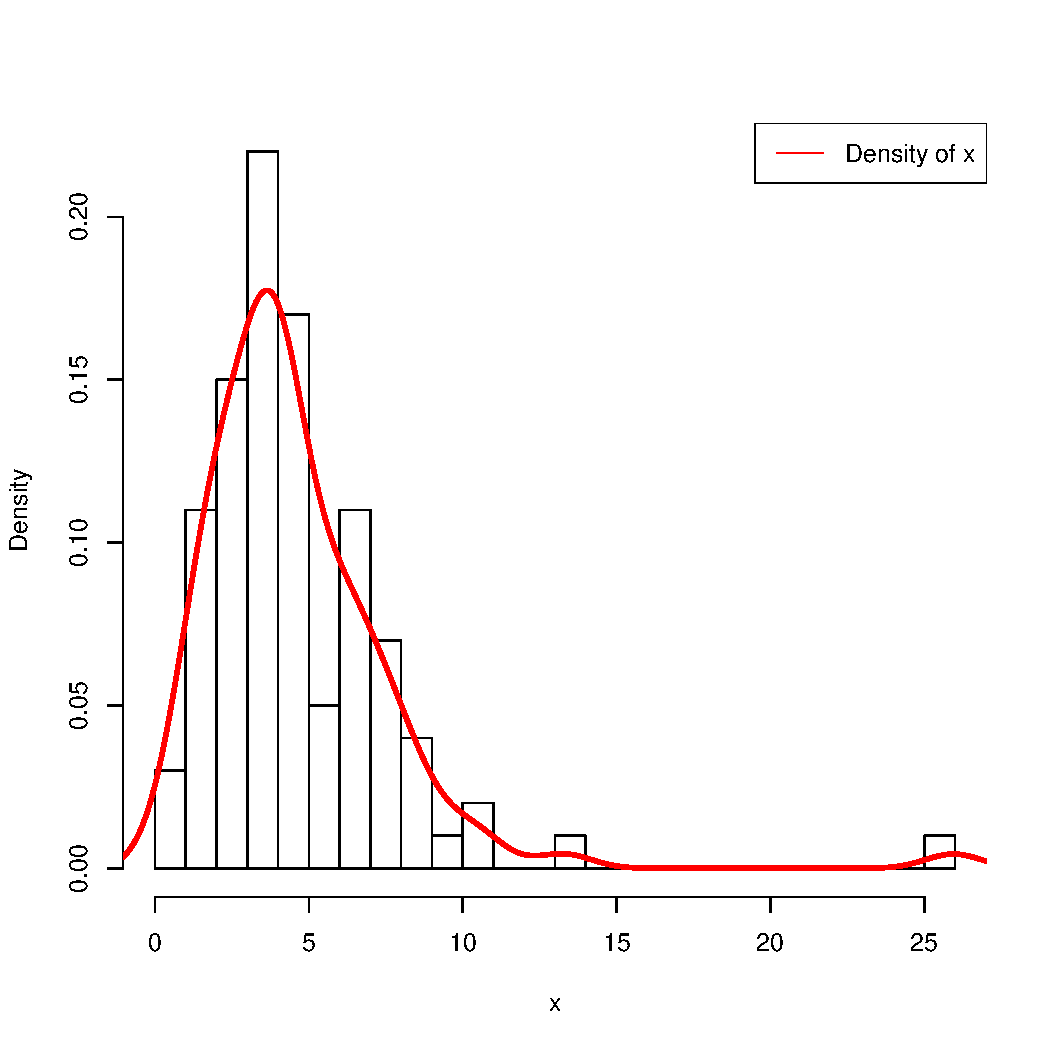
\includegraphics[width = 0.6\linewidth]{plot1.pdf}
  \caption{Sample from mixture gamma}
  \label{p4}
\end{figure}





\begin{figure}[htp]
\centering
  \begin{subfigure}{0.44\textwidth}
  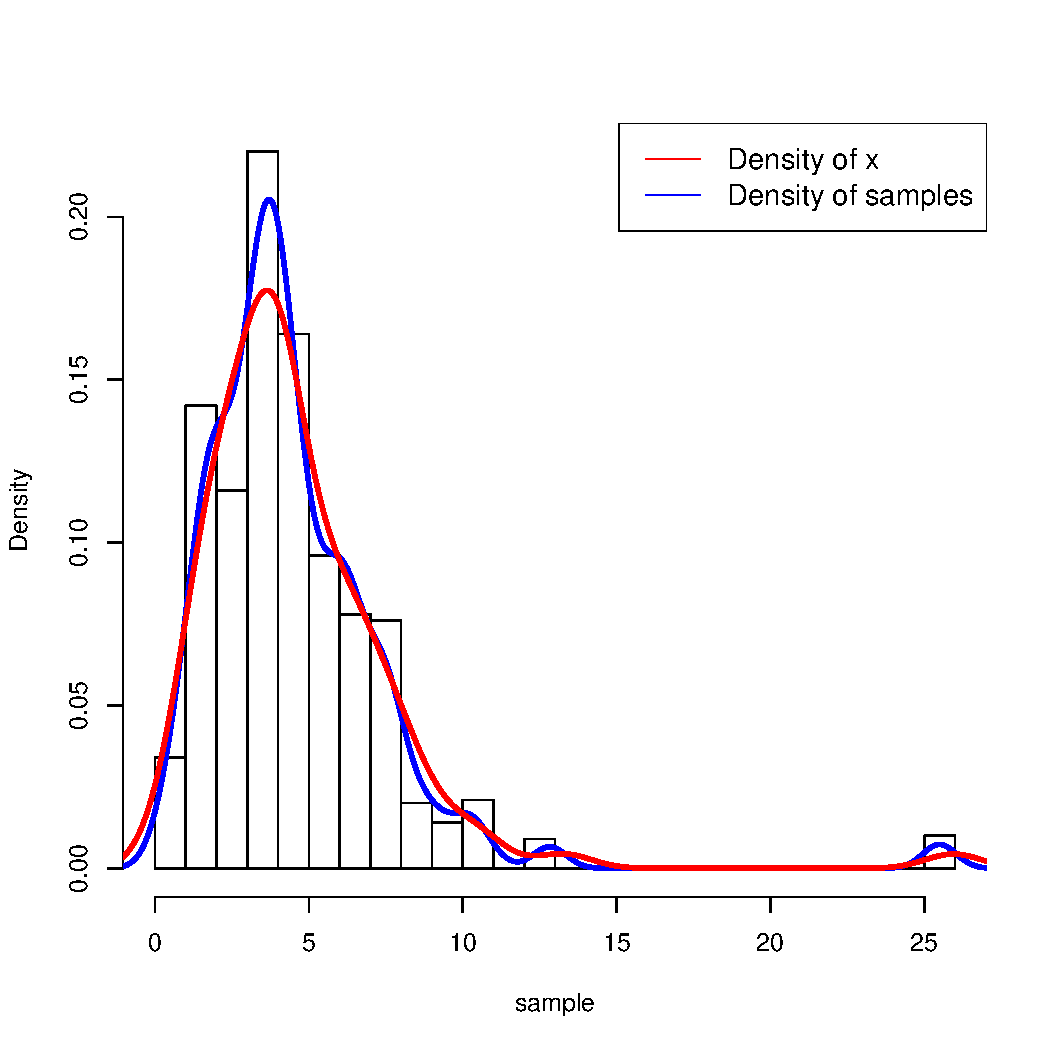
\includegraphics[width=\textwidth]{sample1.pdf}
  \caption{Uniform kernel}
  \end{subfigure}
  \begin{subfigure}{0.44\textwidth}
  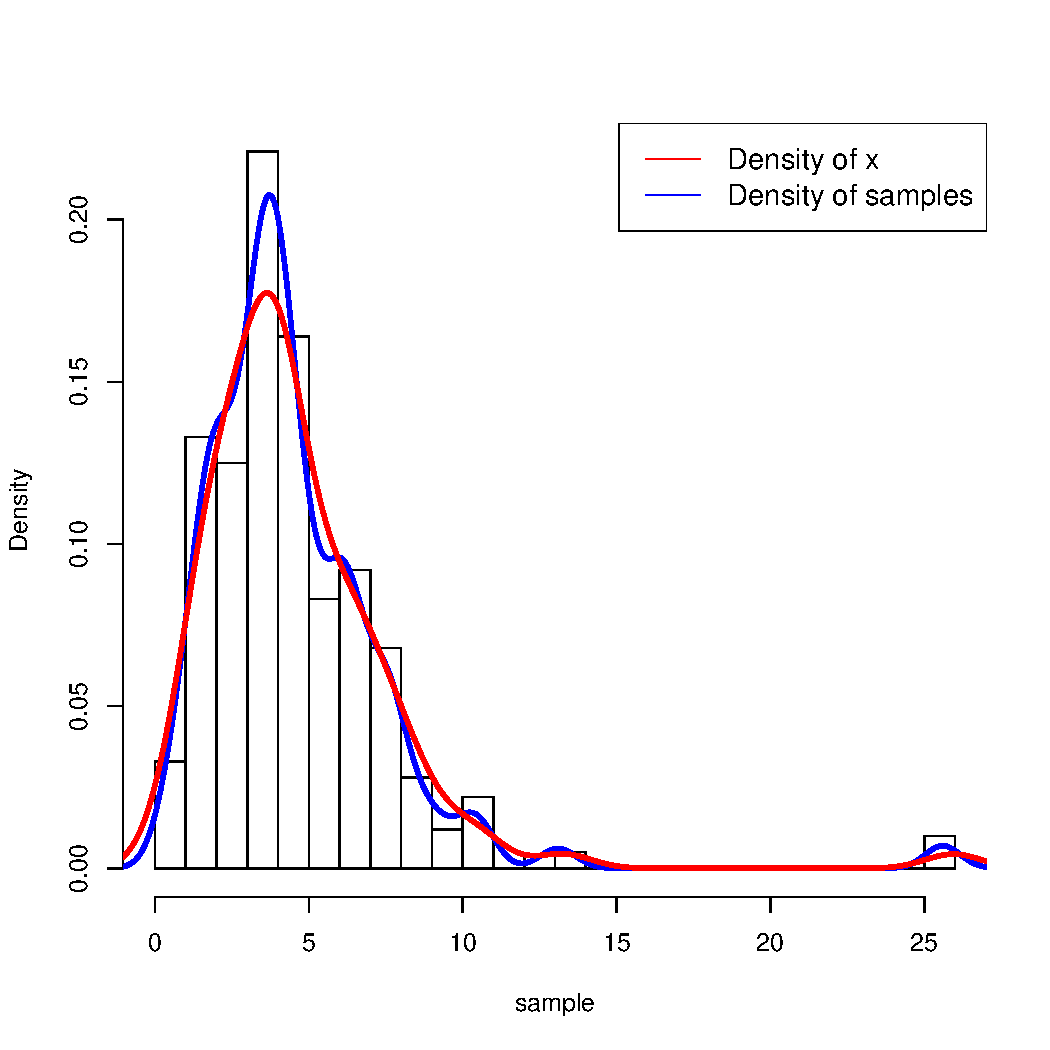
\includegraphics[width=\textwidth]{sample2.pdf}
  \caption{Triangular kernel}
  \end{subfigure}
  \caption{Histogram of samples generated by different kernels.}
  \label{fig:sample_u}
\end{figure}




\subsection{Simulation 2 : Bivariate Case Generate sample from bivariate copula data by kernel density estimator (KDE)}\label{sec:bivariate}
\subsubsection{Generate data from gaussian copula}
The original sample is generated from Copulas because we want the sample to be correlated. Here we use bivariate random variables, $x$, which marginally follows $\text{Gamma}(1,2)$ and $y$, which marginally follows $\chi^2(10)$. Therefore first we use a multivariate Gaussian to generate two correlated random variables, $a$ and $b$, with mean $\left(\begin{matrix} 0 \\ 0 \\ \end{matrix}\right)$ and covariance matrix $\left(\begin{matrix} 1 & 0.5 \\ 0.5 & 1 \\ \end{matrix}\right)$.Then we transform them using the cumulative Gaussian distribution into $u=\Phi(a)$ and $v=\Phi(b)$. Now $u$ and $v$ have marginal uniform distributions and they are still correlated. Finally transform $x = F^{-1}(u)$ and $y= G^{-1}(v)$ where $F(x)$ is the cumulative distribution function of $\text{Gamma}(1,2)$ and $G(y)$ is the cumulative distribution function of $\chi^2(10)$. By this way, we generate data of size $n = 200$ and the plot is shown in figure \ref{p1}.
\begin{figure}[h]
  \centering
  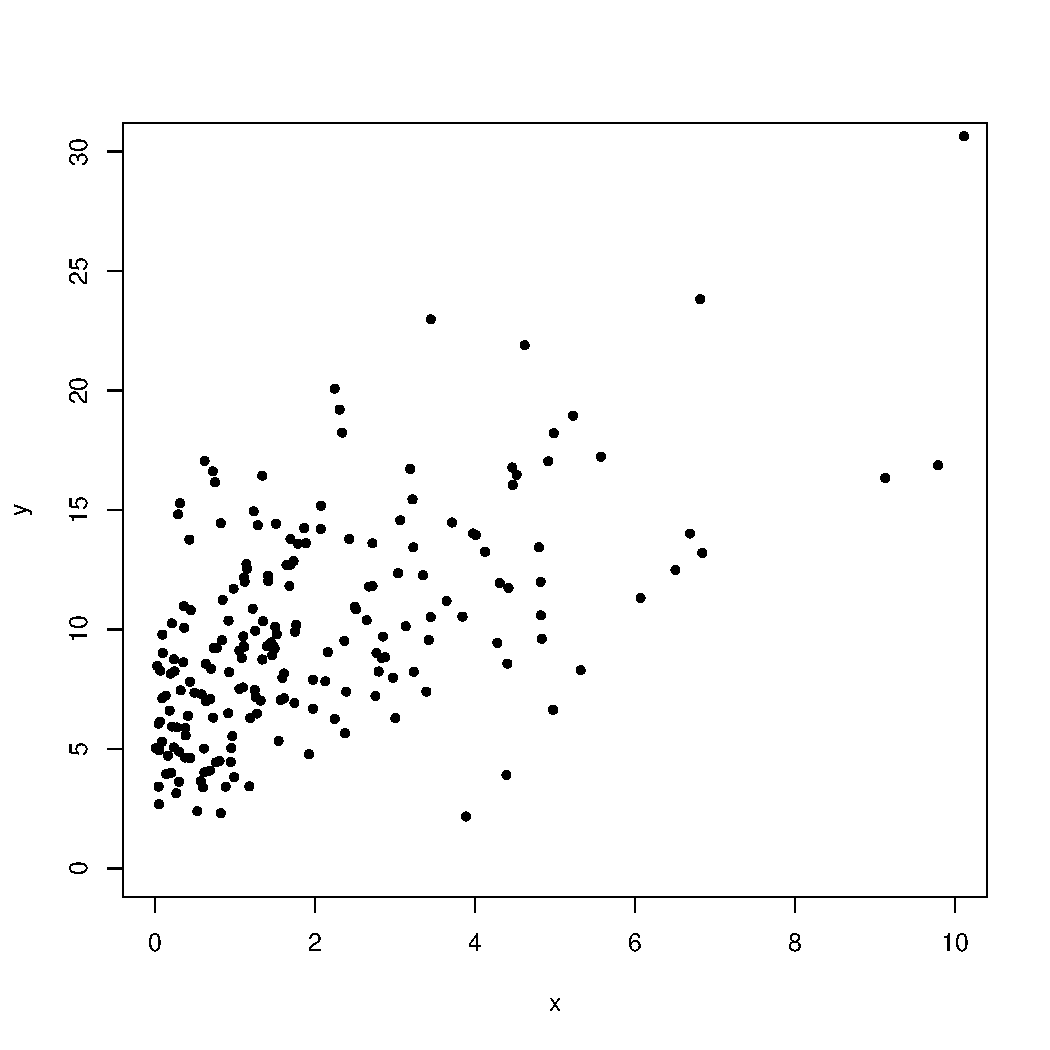
\includegraphics[width = 0.6\linewidth]{plot2.pdf}
  \caption{Data generated from copula.}
  \label{p1}
\end{figure}


\subsubsection{Method 1: Draw sample from Kernel density estimation(KDE)}
The first method is generate random variables inspired by the method of \cite{kde}. As proved in Section \ref{sec:meth}, we first resample from the original data $x$ and $y$ with replacement, and then draw a value from the kernel density, uniform kernel density in our example. The newly generated sample is their summation.
Figure \ref{plot:sp_m} in below shows generated sample using this method for $N = 1000$.


\subsubsection{Method 2: Calculate the kernel density estimation and solve $x = F^{-1}(u)$}
The second method is to construct the kernel density estimation and by equating the CDF of the estimation with $u$, the value draw from uniform (0,1). The sample is solved from the equation $x = F^{-1}(u)$, where $F(\cdot)$ is the CDF of estimated kernel density. Figure \ref{plot:sp_m} in below shows generated sample using KDE for $N = 1000$ using both uniform kernel and triangular kernel.

Figure \ref{plot:sp_m} also gives the plot of samples of size $N = 1000$ generated from true density, which is defined in section \ref{sec:bivariate}. It shows that the samples generated from triangular kernel is the one most close to samples from true density. 



\begin{figure}[htb!]
\centering
\begin{subfigure}{0.45\textwidth}
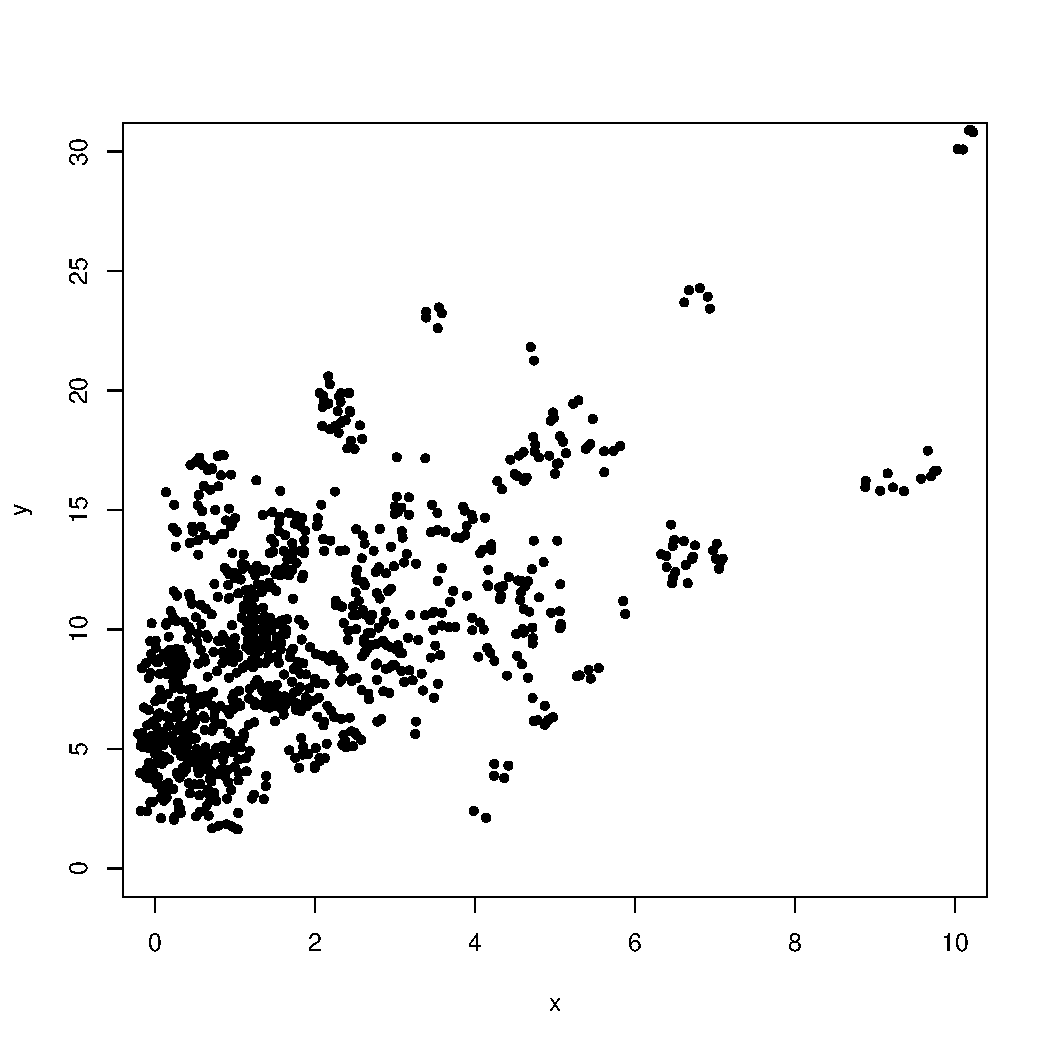
\includegraphics[width = \textwidth]{sample_w.pdf}
\caption{Method 1}
\end{subfigure}
\begin{subfigure}{0.45\textwidth}
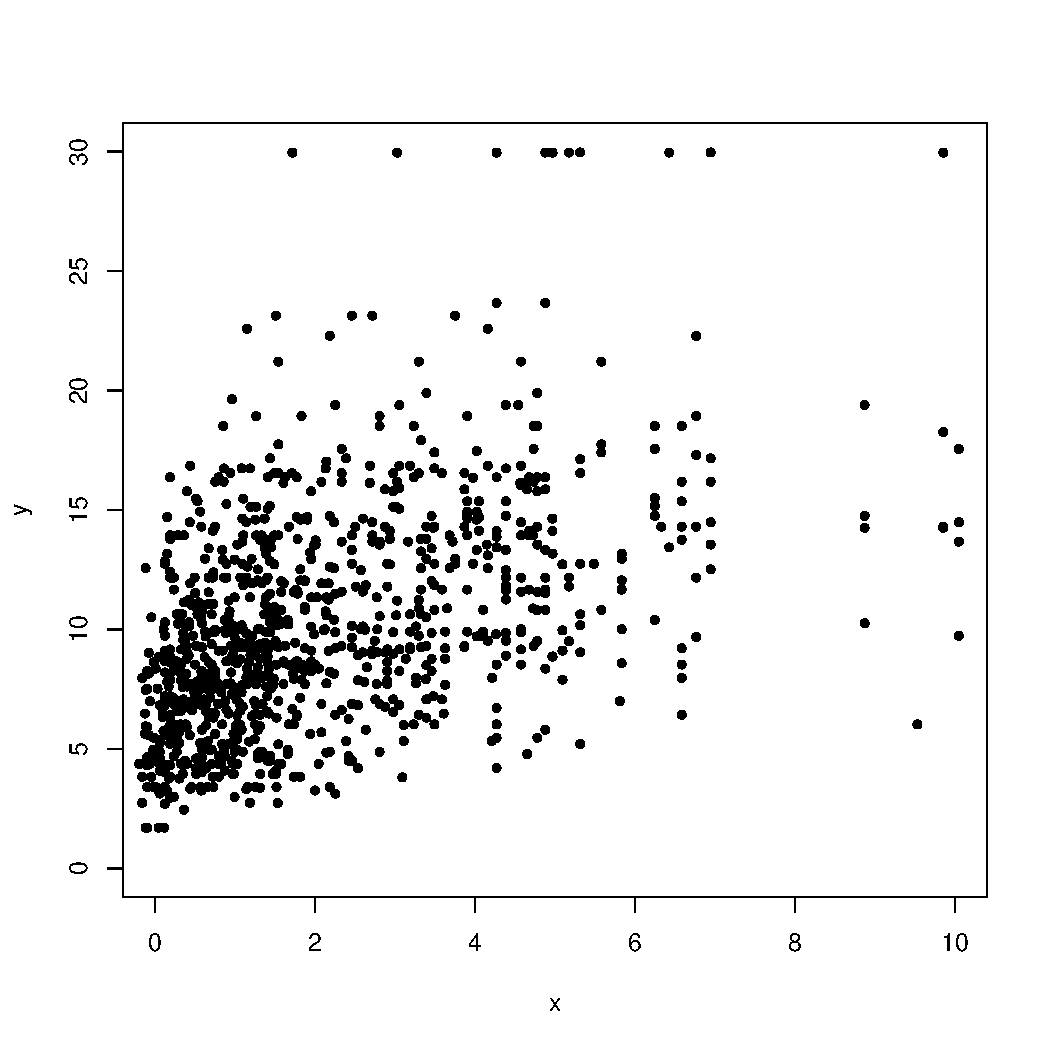
\includegraphics[width = \textwidth]{sample_u.pdf}
\caption{Method 2 : Uniform kernel}
\end{subfigure}
\begin{subfigure}{0.45\textwidth}
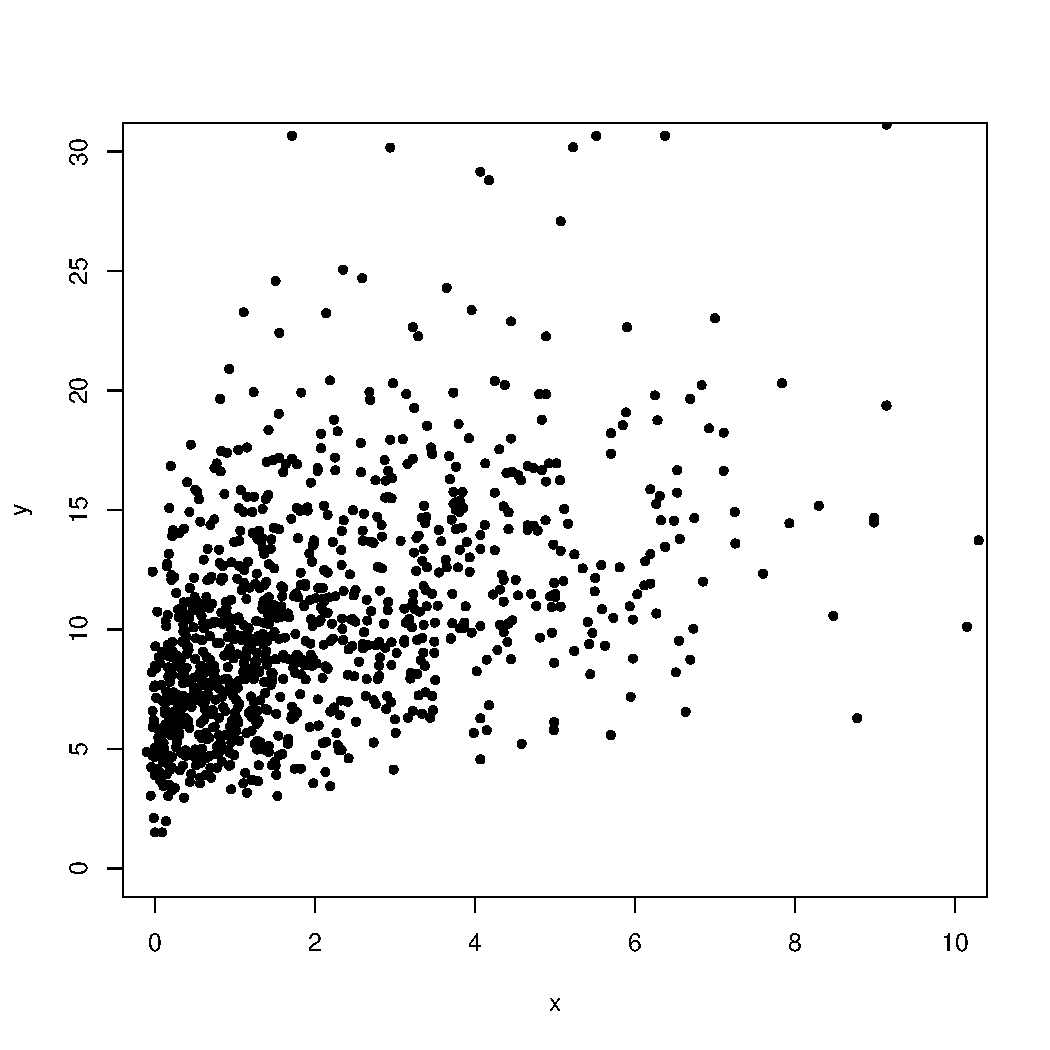
\includegraphics[width = \textwidth]{sample_t.pdf}
\caption{Method 2 : Triangular kernel}
\end{subfigure}
\begin{subfigure}{0.45\textwidth}
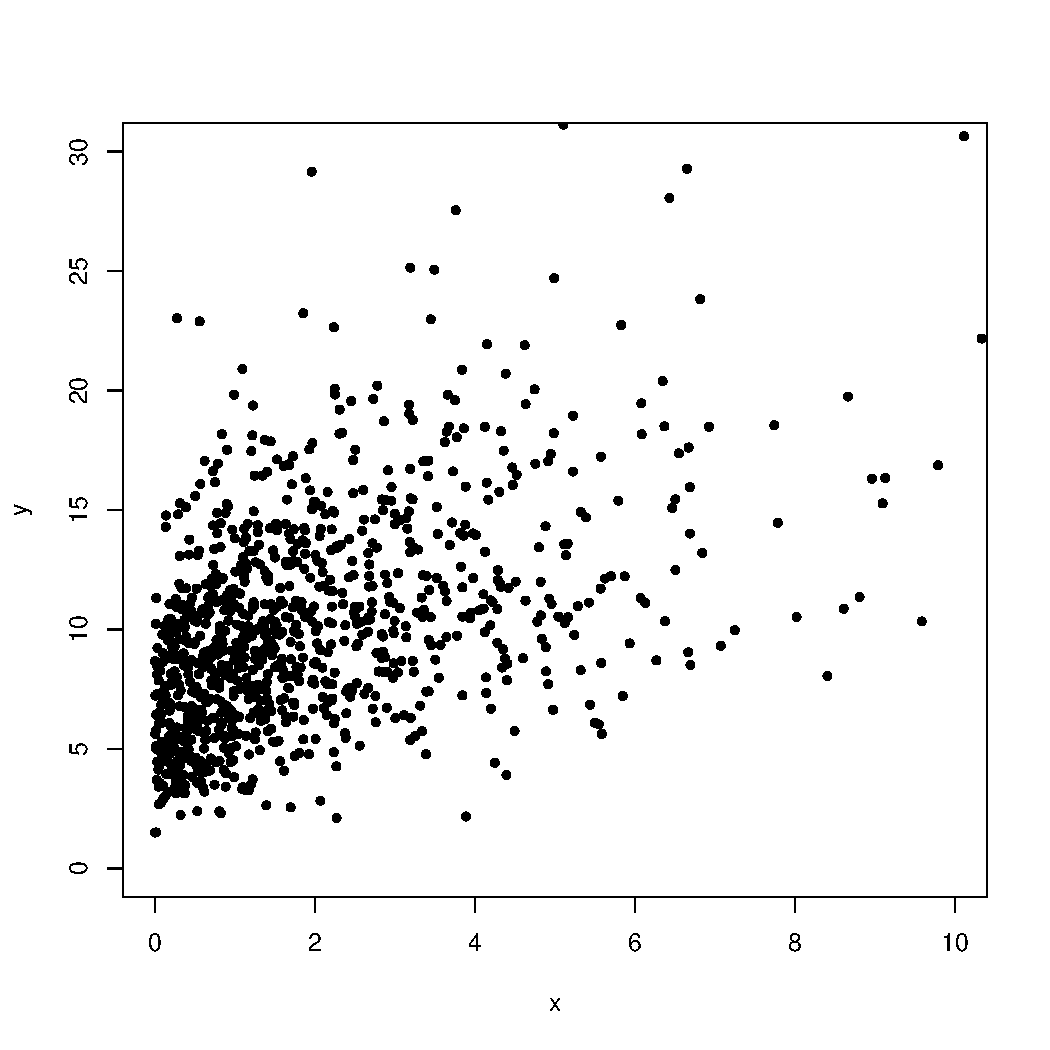
\includegraphics[width = \textwidth]{sample_true.pdf}
\caption{Generate samples from true density}
\end{subfigure}
\caption{Samples generated from different methods.}
\label{plot:sp_m}
\end{figure}



\newpage


\bibliographystyle{plainnat}
\bibliography{citation}

\end{document}

